% This file was created by tikzplotlib v0.9.8.
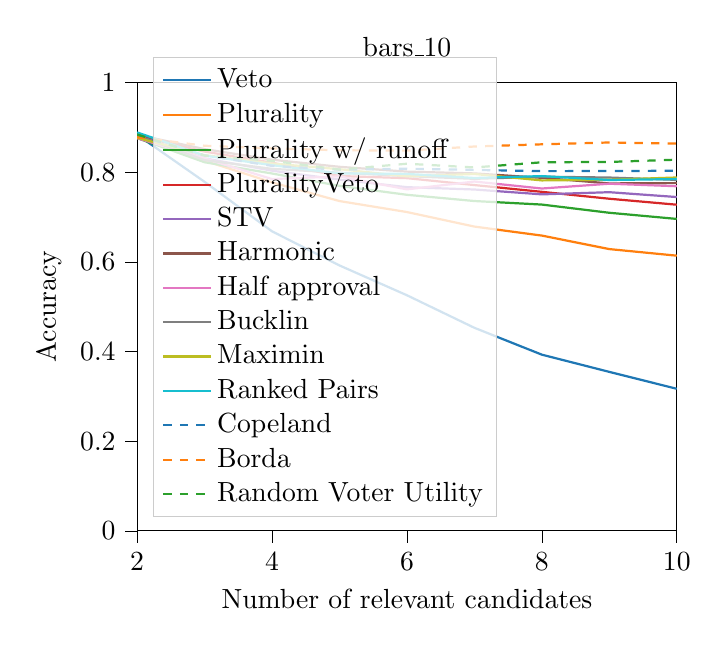
\begin{tikzpicture}

\definecolor{color0}{rgb}{0.12156862745098,0.466666666666667,0.705882352941177}
\definecolor{color1}{rgb}{1,0.498039215686275,0.0549019607843137}
\definecolor{color2}{rgb}{0.172549019607843,0.627450980392157,0.172549019607843}
\definecolor{color3}{rgb}{0.83921568627451,0.152941176470588,0.156862745098039}
\definecolor{color4}{rgb}{0.580392156862745,0.403921568627451,0.741176470588235}
\definecolor{color5}{rgb}{0.549019607843137,0.337254901960784,0.294117647058824}
\definecolor{color6}{rgb}{0.890196078431372,0.466666666666667,0.76078431372549}
\definecolor{color7}{rgb}{0.737254901960784,0.741176470588235,0.133333333333333}
\definecolor{color8}{rgb}{0.0901960784313725,0.745098039215686,0.811764705882353}

\begin{axis}[
legend cell align={left},
legend style={
  fill opacity=0.8,
  draw opacity=1,
  text opacity=1,
  at={(0.03,0.03)},
  anchor=south west,
  draw=white!80!black
},
tick align=outside,
tick pos=left,
title={bars\_10},
x grid style={white!69.0196078431373!black},
xlabel={Number of relevant candidates},
xmin=2, xmax=10,
xtick style={color=black},
y grid style={white!69.0196078431373!black},
ylabel={Accuracy},
ymin=0, ymax=1,
ytick style={color=black}
]
\addplot [thick, color0]
table {%
2 0.8835
3 0.7784
4 0.668
5 0.5919
6 0.5254
7 0.4528
8 0.3929
9 0.3545
10 0.3168
};
\addlegendentry{Veto}
\addplot [thick, color1]
table {%
2 0.8786
3 0.8255
4 0.7772
5 0.7355
6 0.711
7 0.6786
8 0.6585
9 0.6284
10 0.6137
};
\addlegendentry{Plurality}
\addplot [thick, color2]
table {%
2 0.8761
3 0.8221
4 0.797
5 0.7694
6 0.7495
7 0.7356
8 0.7277
9 0.7094
10 0.6957
};
\addlegendentry{Plurality w/ runoff}
\addplot [thick, color3]
table {%
2 0.8812
3 0.8459
4 0.8211
5 0.7914
6 0.7866
7 0.7712
8 0.7561
9 0.7407
10 0.7274
};
\addlegendentry{PluralityVeto}
\addplot [thick, color4]
table {%
2 0.8816
3 0.831
4 0.8032
5 0.7834
6 0.7665
7 0.7613
8 0.7505
9 0.7553
10 0.7445
};
\addlegendentry{STV}
\addplot [thick, color5]
table {%
2 0.8833
3 0.8514
4 0.8278
5 0.8119
6 0.8012
7 0.7972
8 0.7873
9 0.7749
10 0.7756
};
\addlegendentry{Harmonic}
\addplot [thick, color6]
table {%
2 0.8757
3 0.8305
4 0.7846
5 0.7905
6 0.7616
7 0.7791
8 0.7635
9 0.7742
10 0.7686
};
\addlegendentry{Half approval}
\addplot [thick, white!49.8039215686275!black]
table {%
2 0.8818
3 0.8268
4 0.8074
5 0.7988
6 0.7911
7 0.7851
8 0.7899
9 0.788
10 0.7828
};
\addlegendentry{Bucklin}
\addplot [thick, color7]
table {%
2 0.8765
3 0.8381
4 0.8193
5 0.8066
6 0.7907
7 0.7959
8 0.7816
9 0.7831
10 0.7881
};
\addlegendentry{Maximin}
\addplot [thick, color8]
table {%
2 0.8886
3 0.8369
4 0.8155
5 0.7973
6 0.7961
7 0.787
8 0.7912
9 0.7825
10 0.7846
};
\addlegendentry{Ranked Pairs}
\addplot [thick, color0, dashed]
table {%
2 0.8823
3 0.8373
4 0.814
5 0.8055
6 0.8077
7 0.805
8 0.8023
9 0.8024
10 0.8032
};
\addlegendentry{Copeland}
\addplot [thick, color1, dashed]
table {%
2 0.878
3 0.8589
4 0.853
5 0.8488
6 0.848
7 0.8572
8 0.8621
9 0.8662
10 0.8637
};
\addlegendentry{Borda}
\addplot [thick, color2, dashed]
table {%
2 0.884
3 0.8369
4 0.8253
5 0.8057
6 0.8188
7 0.8105
8 0.822
9 0.8228
10 0.8278
};
\addlegendentry{Random Voter Utility}
\end{axis}

\end{tikzpicture}
